\documentclass[12pt,a4paper]{article}
\usepackage{fontspec}
\setmainfont{texgyretermes-regular.otf}[
  BoldFont=texgyretermes-bold.otf,
  ItalicFont=texgyretermes-italic.otf,
  BoldItalicFont=texgyretermes-bolditalic.otf
]
\setmonofont{DejaVuSansMono.ttf}[
  BoldFont=DejaVuSansMono-Bold.ttf,
  ItalicFont=DejaVuSansMono-Oblique.ttf,
  BoldItalicFont=DejaVuSansMono-BoldOblique.ttf,
  Scale=0.84
]

\usepackage[left=2.5cm,right=2.0cm,top=2.5cm,bottom=2.5cm]{geometry}
\setlength{\headheight}{14.5pt}
\addtolength{\topmargin}{-2.5pt}

\usepackage{graphicx}
\usepackage{xcolor}
\usepackage{listings}
\usepackage{titlesec}
\usepackage{fancyhdr}
\usepackage{hyperref}
\usepackage{booktabs}
\usepackage{amsmath,amssymb}
\usepackage{caption}
\usepackage{array}

% Đổi tên các tiêu đề mặc định sang tiếng Việt
\renewcommand{\contentsname}{Mục lục}
\renewcommand{\tablename}{Bảng}
\renewcommand{\figurename}{Hình}

% Định nghĩa màu sắc thương hiệu và code
\definecolor{uitblue}{RGB}{0, 77, 128}
\definecolor{codebg}{RGB}{250, 250, 250}
\definecolor{codeborder}{RGB}{218, 222, 228}
\definecolor{codeblue}{RGB}{0, 75, 175}
\definecolor{codegreen}{RGB}{0, 120, 35}
\definecolor{codered}{RGB}{175, 35, 20}
\definecolor{codegray}{RGB}{115, 115, 115}

% Cấu hình hyperlink
\hypersetup{
    colorlinks=true,
    linkcolor=uitblue,
    filecolor=uitblue,
    urlcolor=uitblue,
    citecolor=uitblue
}

% Cấu hình listings cho Assembly AT&T
\lstdefinelanguage[x86]{AssemblerATnT}{
  morekeywords={
    movl, movb, movw, movzbl, movzwl,
    addl, addb, addw, subl, subb, subw, imull, idivl, divl,
    incl, incb, decl, decb,
    andl, andb, orl, orb, xorl, xorb, notl,
    shll, shrl, sall, sarl,
    cmpl, cmpb, cmpw,
    jmp, je, jne, jb, jbe, ja, jae, jl, jle, jg, jge,
    call, ret, pushl, popl, int,
    .section, .data, .bss, .text, .rodata, .globl, .string, .ascii, .byte, .int, .lcomm, .space
  },
  morecomment=[l]{\#},
  morecomment=[l]{//},
  morestring=[b]",
  morestring=[b]'
}

\lstset{
  language=[x86]{AssemblerATnT},
  backgroundcolor=\color{codebg},
  basicstyle=\ttfamily\scriptsize,
  breaklines=true,
  frame=single,
  rulecolor=\color{codeborder},
  numbers=left,
  numberstyle=\tiny\color{codegray},
  numbersep=7pt,
  tabsize=4,
  keywordstyle=\bfseries\color{codeblue},
  commentstyle=\itshape\color{codegreen},
  stringstyle=\color{codered},
  showstringspaces=false,
  keepspaces=true,
  columns=fullflexible
}

% Cấu hình Header và Footer
\pagestyle{fancy}
\fancyhf{}
\lhead{\small\textit{Thực hành Lập trình Hệ thống}}
\rhead{\small\textit{Lab 02 -- Lập trình Assembly}}
\cfoot{\thepage}
\renewcommand{\headrulewidth}{0.4pt}
\renewcommand{\footrulewidth}{0pt}

% Định dạng tiêu đề section
\titleformat{\section}{\large\bfseries\color{uitblue}}{\thesection}{0.8em}{}
\titleformat{\subsection}{\normalsize\bfseries}{\thesubsection}{0.6em}{}
\titleformat{\subsubsection}{\normalsize\bfseries\itshape}{\thesubsubsection}{0.5em}{}

\begin{document}

% ==================== TRANG BÌA ====================
\begin{titlepage}
    \centering
    \vspace*{-1.0cm}
    {\fontsize{13pt}{16pt}\selectfont ĐẠI HỌC QUỐC GIA THÀNH PHỐ HỒ CHÍ MINH}\\[0.25cm]
    {\fontsize{14pt}{17pt}\selectfont\textbf{TRƯỜNG ĐẠI HỌC CÔNG NGHỆ THÔNG TIN}}\\[0.25cm]
    {\fontsize{12pt}{15pt}\selectfont\textbf{KHOA MẠNG MÁY TÍNH VÀ TRUYỀN THÔNG}}\\[1.0cm]

    
\includegraphics[width=4.8cm]{images/uit_logo.png}\\[1.2cm]

    {\color{uitblue}\rule{\textwidth}{1.6pt}}\\[0.6cm]
    {\fontsize{22pt}{26pt}\selectfont\textbf{BÁO CÁO THỰC HÀNH}}\\[0.4cm]
    {\fontsize{16pt}{20pt}\selectfont\textbf{LAB 02: LẬP TRÌNH ASSEMBLY CƠ BẢN}}\\[0.3cm]
    {\fontsize{13pt}{16pt}\selectfont\textit{Basic Assembly Programming -- Lập trình hợp ngữ x86}}\\[0.4cm]
    {\color{uitblue}\rule{\textwidth}{1.6pt}}\\[2.0cm]

    \begin{minipage}{0.75\textwidth}
        \fontsize{12pt}{17pt}\selectfont
        \begin{tabular}{ll}
            \textbf{Nhóm:} & Nhóm 4 \\[0.2cm]
            \textbf{Sinh viên 1:} & Bùi Thái Sơn \quad -- 25521588 \\[0.2cm]
            \textbf{Sinh viên 2:} & Võ Quốc Thịnh \quad -- 25521787 \\[0.2cm]
            \textbf{Sinh viên 3:} & Lê Thành Đạt \quad -- 25520270
        \end{tabular}
    \end{minipage}

    \vfill
    {\fontsize{12pt}{15pt}\selectfont Thành phố Hồ Chí Minh, tháng 10 năm 2026}
\end{titlepage}

% ==================== MỤC LỤC ====================
\thispagestyle{empty}
\tableofcontents
\newpage
\setcounter{page}{1}

% ==================== PHẦN 1 ====================
\section{Chi tiết các bài tập và giải thích mã nguồn}

% ==================== BÀI 2.1 ====================
\subsection{Bài 2.1: In ra độ dài của chuỗi cho trước (tối đa 9 ký tự)}

\textbf{Yêu cầu đề bài:}
Cho trước một chuỗi ký tự \texttt{msg} được định nghĩa trong \texttt{.section .data} (độ dài tối đa 9 ký tự). Hãy viết chương trình hợp ngữ tính độ dài chuỗi (không tính ký tự null kết thúc chuỗi \texttt{\textbackslash 0}) và in giá trị này ra màn hình kèm ký tự xuống dòng.

\textbf{Giải thích mã nguồn:}
Chương trình xác định trước độ dài chuỗi cố định \texttt{msg} ngay ở giai đoạn hợp dịch thông qua biểu thức \texttt{msg\_len = . - msg - 1}, lấy vị trí hiện tại trừ địa chỉ đầu chuỗi và trừ bỏ 1 byte null \texttt{\textbackslash 0}. Giá trị số này được cộng với \texttt{0x30} để chuyển đổi trực tiếp sang ký tự chữ số ASCII rồi lưu sẵn cùng mã xuống dòng \texttt{0x0a} trong vùng nhớ \texttt{output}. Khi khởi chạy, chương trình chỉ cần nạp địa chỉ buffer vào \texttt{\%ecx}, độ dài 2 bytes vào \texttt{\%edx} và gọi \texttt{sys\_write} (\texttt{\%eax = 4}) ra \texttt{stdout} (\texttt{\%ebx = 1}) qua ngắt \texttt{int \$0x80}, sau đó thoát tiến trình an toàn bằng \texttt{sys\_exit}.


\textbf{Mã nguồn chương trình (\texttt{bai2.1.s}):}
\begin{lstlisting}
.section .data
msg:
	.string "IloveCR7"
msg_len = . - msg - 1 # Lay dia chi hien tai - dia chi msg - 1 (tru byte null)

output:
	.byte msg_len + 0x30 # Cong 48 (0x30) de chuyen thanh ky tu ASCII
	.byte 0x0a           # Ky tu xuong dong '\n'

.section .text
	.globl _start
_start:
	movl $output, %ecx   # Dia chi buffer can xuat
	movl $0x2, %edx      # Do dai xuat ra: 2 bytes
	movl $0x1, %ebx      # File descriptor: stdout (1)
	movl $0x4, %eax      # System call number: sys_write (4)
	int $0x80            # Goi kernel xuat chuoi

	movl $0x1, %eax      # System call number: sys_exit (1)
	int $0x80            # Thoat chuong trinh
\end{lstlisting}

% ==================== BÀI 2.2 ====================
\subsection{Bài 2.2: Tính số dư của tổng 4 số có 2 chữ số khi chia 8}

\textbf{Yêu cầu đề bài:}
Nhập lần lượt 4 số nguyên có 2 chữ số ($10 \le x \le 99$) từ bàn phím. Tính tổng 4 số đã nhập và in ra màn hình số dư của tổng khi chia cho 8.

\textbf{Giải thích mã nguồn:}
Chương trình tách tác vụ nhập liệu thành thủ tục con \texttt{nhapso} và gọi 4 lần liên tiếp để nhận lần lượt 4 số từ người dùng qua \texttt{sys\_read}. Mỗi số đọc được gồm 2 ký tự số được chuyển đổi về giá trị nguyên bằng cách trừ 48, lấy chữ số đầu nhân 10 rồi cộng với chữ số sau trước khi cộng dồn vào biến \texttt{ans}. Sau khi hoàn tất nhập liệu, thủ tục \texttt{inkq} xóa thanh ghi \texttt{\%edx}, nạp tổng vào \texttt{\%eax} và thực hiện phép chia không dấu 64-bit cho 8 bằng lệnh \texttt{divl \%ecx}. Phần dư nằm trong \texttt{\%edx} được cộng thêm 48 thành mã ASCII và in ra màn hình cùng chuỗi thông báo qua \texttt{sys\_write}.


\textbf{Mã nguồn chương trình (\texttt{bai2\_2.s}):}
\begin{lstlisting}
.section .data
nhapvao:
	.string  "Enter a number (2-digit): "
kq:
	.string "Remainder: "
newline:
	.byte 10
ans:
	.int 0

.section .bss
	.lcomm number1, 4

.section .text
	.globl _start

jmp _start

nhapso:
	movl $4, %eax        # sys_write in loi nhac
	movl $1, %ebx
	movl $nhapvao, %ecx
	movl $26, %edx
	int $0x80

	movl $3, %eax        # sys_read doc 3 bytes tu STDIN
	movl $0, %ebx
	movl $number1, %ecx
	movl $3, %edx
	int $0x80

	movzbl number1, %eax    # Doc chu so hang chuc
	subl $48, %eax          # Chuyen thanh gia tri nguyen
	imull $10, %eax         # Nhan voi 10

	movzbl number1+1, %ebx  # Doc chu so hang don vi
	subl $48, %ebx
	addl %ebx, %eax         # Tong gia tri cua so vua nhap

	addl %eax, ans          # Cong don vao bien tong ans
	ret

inkq:
	movl ans, %eax       # Nap tong vao %eax
	xorl %edx, %edx      # Xoa %edx de chuan bi chia 64-bit
	movl $8, %ecx        # So chia = 8
	divl %ecx            # Chia: thuong o %eax, so du o %edx

	movl %edx, ans
	addl $48, ans        # Chuyen so du sang ky tu ASCII

	movl $4, %eax        # In chuoi thong bao "Remainder: "
	movl $1, %ebx
	movl $kq, %ecx
	movl $11, %edx
	int $0x80

	movl $4, %eax        # In ky tu so du
	movl $1, %ebx
	movl $ans, %ecx
	movl $1, %edx
	int $0x80

	movl $4, %eax        # In dau xuong dong
	movl $1, %ebx
	movl $newline, %ecx
	movl $1, %edx
	int $0x80
	ret

_start:
	call nhapso
	call nhapso
	call nhapso
	call nhapso
	call inkq

	mov $1, %eax         # sys_exit
	int $0x80
\end{lstlisting}

% ==================== BÀI 2.3 ====================
\subsection{Bài 2.3: Mã hóa Caesar trên một chuỗi ký tự (Cơ bản + Nâng cao 1 \& 2)}

\textbf{Yêu cầu đề bài:}
\begin{itemize}
    \item \textbf{Cơ bản:} Nhập một chuỗi ký tự và số bước dịch $n$ ($0 \le n \le 9$), xuất ra chuỗi đã được mã hóa Caesar tương ứng.
    \item \textbf{Nâng cao 1:} Xử lý xoay vòng chuẩn khi ký tự sau khi dịch vượt quá \texttt{'z'} hoặc \texttt{'Z'} (ví dụ: với $n=3$, \texttt{'z'} chuyển thành \texttt{'c'}).
    \item \textbf{Nâng cao 2:} Hỗ trợ đồng thời cả chữ in hoa (\texttt{'A'}--\texttt{'Z'}) và chữ in thường (\texttt{'a'}--\texttt{'z'}). Tất cả ký tự số, ký tự đặc biệt, khoảng trắng được giữ nguyên không đổi. Chuỗi đầu vào có độ dài tùy chọn tối đa 255 ký tự.
\end{itemize}

\textbf{Giải thích mã nguồn:}
Sau khi đọc chuỗi văn bản (tối đa 255 ký tự) và số bước dịch $n \in [0, 9]$, chương trình duyệt con trỏ \texttt{\%edx} qua từng byte của bộ đệm để tiến hành mã hóa. Tại mỗi bước, nếu ký tự thuộc bảng chữ cái tiếng Anh, chương trình xác định mốc cơ sở (\texttt{'A'} cho chữ hoa hoặc \texttt{'a'} cho chữ thường) rồi đưa mã về khoảng giá trị $0..25$, cộng thêm $n$, và tự động xoay vòng bằng cách trừ đi 26 nếu bị tràn trước khi chuyển ngược lại mã ASCII gốc. Toàn bộ chữ số, khoảng trắng và ký tự đặc biệt được giữ nguyên vẹn mà không làm thay đổi định dạng văn bản gốc, sau đó kết quả được xuất ra màn hình qua \texttt{sys\_write}.


\textbf{Mã nguồn chương trình (\texttt{bai2.3.s}):}
\begin{lstlisting}
.section .rodata
enter_string:
    .ascii "Enter a string (<255 chars): "
enter_string_len = .-enter_string

shift_string:
    .ascii "Enter n (0-9): "
shift_string_len = .-shift_string

.section .bss
    .lcomm input_str, 256
    .lcomm input_len, 4
    .lcomm n, 2

.section .text
	.globl _start

printf:
	movl $0x1, %ebx         # stdout
	movl $0x4, %eax         # write
	int $0x80
	ret

read:
	xorl %ebx, %ebx         # stdin
	movl $0x3, %eax         # read
	int $0x80
	ret

cipher:
	movl $0, %ecx
	movl $input_str, %edx
	decl %edx

.cipher_loop:
	cmpl input_len, %ecx
	je .fin
	incl %edx
	incl %ecx
	cmpb $'A', (%edx)
	jb .cipher_loop     # Ky tu ngoai khoang (giu nguyen)
	cmpb $'Z', (%edx)
	movb $'A', %bl
	jbe .shift          # Chu hoa ('A' <= x <= 'Z')

	cmpb $'a', (%edx)
	jb .cipher_loop     # Ky tu dac biet nam giua 'Z' va 'a'
	cmpb $'z', (%edx)
	movb $'a', %bl
	jbe .shift          # Chu thuong ('a' <= x <= 'z')

	jmp .cipher_loop    # Ky tu lon hon 'z'

.fin:
	ret

.shift:
	movb (%edx), %al
	subb %bl, %al       # Dua ve khoang 0 .. 25
	addb n, %al         # Cong buoc dich n
	cmpb $26, %al       # Kiem tra tran 26
	jb .done
	subb $26, %al       # Xoay vong bang cach tru 26

.done:
	addb %bl, %al       # Dua ve lai ma ASCII goc
	movb %al, (%edx)    # Ghi de ky tu da ma hoa vao buffer
	jmp .cipher_loop

_start:
	movl $enter_string, %ecx
	movl $enter_string_len, %edx
	call printf

	movl $input_str, %ecx
	movl $256, %edx
	call read
	movl %eax, input_len

	movl $shift_string, %ecx
	movl $shift_string_len, %edx
	call printf

	movl $n, %ecx
	movl $0x2, %edx
	call read
	subb $0x30, n
	call cipher

	movl $input_str, %ecx
	movl input_len, %edx
	call printf

	movl $1, %eax
	int $0x80
\end{lstlisting}

% ==================== BÀI 2.4 ====================
\subsection{Bài 2.4: Đếm số lượng bội của 10 trong khoảng [x, y]}

\textbf{Yêu cầu đề bài:}
Nhập từ bàn phím hai số nguyên có 2 chữ số $x$ và $y$ ($10 \le x \le y \le 99$). Đếm số lượng các số chia hết cho 10 nằm trong đoạn đóng $[x, y]$ (tính cả $x$ và $y$).

\textbf{Giải thích mã nguồn:}
Thay vì sử dụng vòng lặp duyệt tốn kém, chương trình áp dụng công thức toán học $O(1)$ để tính số lượng bội của 10 trong đoạn đóng $[x, y]$ thông qua hiệu số $\lfloor y/10 \rfloor - \lfloor (x - 1)/10 \rfloor$. Hai chuỗi 2 chữ số $x$ và $y$ nhập từ bàn phím được chuyển đổi sang số nguyên; $x$ giảm đi 1 rồi chia 10 lấy thương lưu vào \texttt{\%edi}, còn $y$ chia 10 lấy thương lưu vào \texttt{\%esi}. Hiệu số giữa hai thương được cộng thêm \texttt{'0'} thành ký tự ASCII, đẩy trực tiếp lên đỉnh ngăn xếp (\texttt{pushl \%esi}) và tận dụng địa chỉ con trỏ đỉnh ngăn xếp \texttt{\%esp} làm bộ nhớ đệm để xuất kết quả ra màn hình mà không cần cấp phát thêm biến.


\textbf{Mã nguồn chương trình (\texttt{bai2.4.s}):}
\begin{lstlisting}
.section .data
hihi:
	.string "Nhap so: "
string_len = . - hihi
newline:
	.ascii "\n"

.section .bss
	.lcomm x, 3
	.lcomm y, 3

.section .text
.globl _start

_start:
	# 1. Nhap va tinh [(x - 1) / 10]
	movl $4, %eax
	movl $1, %ebx
	movl $hihi, %ecx
	movl $string_len, %edx
	int $0x80
	
	movl $0, %ebx
	movl $3, %eax
	movl $x, %ecx
	movl $3, %edx
	int $0x80
	
	movzbl x, %edi
	subl $'0', %edi
	imull $10, %edi
	
	movzbl x+1, %eax
	subl $'0', %eax
	addl %eax, %edi
	
	decl %edi            # Tinh x - 1
	movl $10, %ecx
	movl %edi, %eax
	xorl %edx, %edx
	divl %ecx            # Chia 10: thuong nam o %eax
	movl %eax, %edi      # Luu [(x - 1) / 10] vao %edi

	# 2. Nhap va tinh [y / 10]
	movl $4, %eax
	movl $1, %ebx
	movl $hihi, %ecx
	movl $string_len, %edx 
	int $0x80

	movl $0, %ebx
	movl $3, %eax
	movl $y, %ecx
	movl $3, %edx
	int $0x80

	movzwl y, %eax
	subb $'0', %al
	subb $'0', %ah

	movzbl %al, %ecx
	imull $10, %ecx
	movzbl %ah, %edx
	addl %edx, %ecx      # y gio nam o %ecx
	
	movl %ecx, %eax	
	movl $10, %ecx
	xorl %edx, %edx
	divl %ecx            # Chia 10: thuong o %eax
	movl %eax, %esi      # Luu [y / 10] vao %esi

	# 3. Tinh hieu so va xuat ket qua
	subl %edi, %esi      # %esi = [y/10] - [(x-1)/10]
	addl $'0', %esi      # Chuyen thanh ky tu ASCII
	pushl %esi           # Day vao dinh ngan xep
	
	movl $4, %eax
	movl $1, %ebx
	movl %esp, %ecx      # Dung dia chi %esp lam buffer xuat
	movl $1, %edx
	int $0x80

	movl $4, %eax        # Xuat dau xuong dong
	movl $1, %ebx
	movl $newline, %ecx
	movl $1, %edx
	int $0x80

	movl $1, %eax        # Thoat
	xorl %ebx, %ebx
	int $0x80
\end{lstlisting}

% ==================== BÀI 2.5 ====================
\subsection{Bài 2.5: Kiểm tra tuổi đoàn dựa vào năm sinh (Cơ bản + Nâng cao)}

\textbf{Yêu cầu đề bài:}
\begin{itemize}
    \item \textbf{Cơ bản:} Nhập năm sinh có 4 chữ số từ bàn phím. Nếu tuổi từ 16 đến 30 tuổi thì xuất thông báo \texttt{"Thuoc Doan TN"}, ngược lại xuất \texttt{"Khong thuoc Doan TN"}.
    \item \textbf{Nâng cao:} Xuất kèm theo số tuổi cụ thể tính được (ví dụ: \texttt{"Tuoi: 21"}).
\end{itemize}

\textbf{Giải thích mã nguồn:}
Chương trình nhận chuỗi năm sinh 4 chữ số, tính giá trị nguyên theo trọng số hàng nghìn, trăm, chục, đơn vị rồi lấy mốc năm 2026 trừ đi để xác định tuổi. Tiếp theo, lệnh \texttt{cmpl} rẽ nhánh kiểm tra: nếu tuổi nằm ngoài khoảng $[16, 30]$ thì in thông báo \texttt{"Khong thuoc Doan TN"}, ngược lại in \texttt{"Thuoc Doan TN"}. Đối với yêu cầu nâng cao, thủ tục \texttt{print} chia liên tiếp số tuổi cho 10, đẩy từng phần dư (mã ASCII) vào ngăn xếp theo cơ chế LIFO rồi lần lượt rút ra xuất ra màn hình, giúp hiển thị chính xác số tuổi nhiều chữ số theo đúng thứ tự mà không cần đảo chuỗi thủ công.


\textbf{Mã nguồn chương trình (\texttt{bai2.5.s}):}
\begin{lstlisting}
.section .data
hello:
	.ascii "Nhap nam sinh: "
string_len = . - hello

Thuoc:
	.ascii "Thuoc Doan TN\n"
Thuoc_len = . - Thuoc

Khongthuoc:
	.ascii "Khong thuoc Doan TN\n"
Khongthuoc_len = . - Khongthuoc

intuoi:
	.ascii "Tuoi: "
intuoi_len = . - intuoi

newline:
	.ascii "\n"

.section .bss
	.lcomm tuoi, 5
	.lcomm out, 1

.section .text
.globl _start

_start:
	# 1. Nhap nam sinh tu ban phim
	movl $4, %eax
	movl $1, %ebx
	movl $hello, %ecx
	movl $string_len, %edx
	int $0x80

	movl $3, %eax
	movl $0, %ebx
	movl $tuoi, %ecx
	movl $5, %edx
	int $0x80

	# 2. Chuyen 4 ky tu thanh so nguyen trong %edi
	xorl %edi, %edi
		
	movzbl tuoi, %eax
	subl $'0', %eax
	imull $1000, %eax
	addl %eax, %edi
	
	movzbl tuoi+1, %eax
	subl $'0', %eax
	imull $100, %eax 
	addl %eax, %edi

	movzbl tuoi+2, %eax
	subl $'0', %eax
	imull $10, %eax 
	addl %eax, %edi

	movzbl tuoi+3, %eax
	subl $'0', %eax 
	addl %eax, %edi

	# 3. Tinh tuoi: 2026 - nam_sinh
	movl $2026, %eax
	subl %edi, %eax
	movl %eax, %edi
	
	# 4. Kiem tra khoang [16, 30]
	cmpl $16, %edi
	jl ngoai_khoang
	cmpl $30, %edi
	jg ngoai_khoang
	
	movl $4, %eax
	movl $1, %ebx
	movl $Thuoc, %ecx
	movl $Thuoc_len, %edx
	int $0x80
	jmp nang_cao

ngoai_khoang:
	movl $4, %eax
	movl $1, %ebx
	movl $Khongthuoc, %ecx
	movl $Khongthuoc_len, %edx
	int $0x80

nang_cao:
	movl $4, %eax
	movl $1, %ebx
	movl $intuoi, %ecx
	movl $intuoi_len, %edx
	int $0x80
	call print

done:
	movl $1, %eax
	xorl %ebx, %ebx
	int  $0x80

# Thu tuc print: in so nguyen trong %edi ra man hinh
print:
	movl %edi, %eax
	xorl %esi, %esi

chia_loop:
	xorl %edx, %edx
	movl $10, %ebx
	divl %ebx            # Chia 10 lay so du vao %edx
	addb $'0', %dl       # Chuyen sang ma ASCII
	pushl %edx           # Day vao ngan xep
	incl %esi            # Tang bien dem chu so
	cmpl $0, %eax
	jne chia_loop

in_loop:
	popl %eax            # Rut chu so theo thu tu dung
	movb %al, out
	movl $4, %eax
	movl $1, %ebx
	movl $out, %ecx
	movl $1, %edx
	int $0x80
	decl %esi
	jnz in_loop

	movl $4, %eax        # In ky tu xuong dong
	movl $1, %ebx
	movl $newline, %ecx
	movl $1, %edx
	int $0x80
	ret
\end{lstlisting}

% ==================== BÀI 2.6 ====================
\subsection{Bài 2.6: Kiểm tra năm nhuận (Cơ bản + Nâng cao)}

\textbf{Yêu cầu đề bài:}
\begin{itemize}
    \item \textbf{Cơ bản:} Nhập một năm $a$ có 4 chữ số ($1000 \le a \le 9999$). Xuất ra \texttt{"Nam nhuan"} nếu là năm nhuận, ngược lại xuất \texttt{"Nam khong nhuan"}.
    \item \textbf{Nâng cao:} Tìm và in ra năm nhuận kế tiếp sau năm vừa nhập.
\end{itemize}

\textbf{Giải thích mã nguồn:}
Chương trình đọc năm 4 chữ số và kiểm tra tính nhuận theo quy tắc lịch Gregory: nếu hai chữ số cuối bằng \texttt{00} (năm tròn thế kỷ), chương trình chia cho 400; nếu khác \texttt{00}, chương trình chỉ cần chia 4 hai chữ số cuối để đưa ra kết luận \texttt{"Nam nhuan"} hoặc \texttt{"Nam khong nhuan"}. Tiếp đó, hàm \texttt{namnhuantieptheo} liên tục tăng giá trị năm lên 1 và lặp lại kiểm tra chia hết cho 4, 100 và 400 cho đến khi tìm được năm nhuận kế tiếp. Giá trị năm tìm được được chuyển đổi ngược thành chuỗi bằng cách chia 10 lấy dư và ghi lùi từ cuối bộ đệm \texttt{buffer\_num} về trước rồi xuất ra màn hình.


\textbf{Mã nguồn chương trình (\texttt{bai2\_6.s}):}
\begin{lstlisting}
.section .data
nhapvao:
	.string  "Enter a year (4-digit): "
kqnamnhuan:
	.string "Nam nhuan\n"
kqnamkhongnhuan:
	.string "Nam khong nhuan\n"
namnhuantieptheouwu:
	.string "Nam nhuan ke tiep: "
newline:
	.byte 10
ans:
	.int 0

.section .bss
	.lcomm number1, 5
	buffer_num: .space 16

.section .text
	.globl _start

jmp _start

namnhuantieptheo:
	addl $1, ans         # Tang nam len 1
	movl ans, %eax
	xorl %edx, %edx
	movl $4, %ecx
	divl %ecx
	cmpl $0, %edx 
	jne namnhuantieptheo # Khong chia het cho 4 -> lap tiep
    
	movl ans, %eax
	xorl %edx, %edx
	movl $100, %ecx
	divl %ecx
	cmpl $0, %edx
	jne okroido          # Chia het cho 4 va khong chia het cho 100 -> Nam nhuan!

	movl ans, %eax
	xorl %edx, %edx
	movl $400, %ecx
	divl %ecx
	cmpl $0, %edx
	jne namnhuantieptheo # Chia het cho 100 nhung khong chia het cho 400 -> Lap tiep
    
okroido:
	movl $4, %eax
	movl $1, %ebx
	movl $namnhuantieptheouwu, %ecx
	movl $19, %edx
	int $0x80

	movl ans, %eax
	movl $buffer_num + 10, %esi
	movl $0, %ecx

chuyen_doi:
	decl %esi
	xorl %edx, %edx
	movl $10, %ebx
	divl %ebx
	addb $48, %dl
	movb %dl, (%esi)
	incl %ecx
	cmpl $0, %eax
	jne chuyen_doi

	movl $4, %eax
	movl $1, %ebx
	movl %esi, %ecx
	movl $buffer_num + 10, %edx
	subl %esi, %edx
	int $0x80

	call xuonghang
	ret

xuonghang:
	movl $4, %eax
	movl $1, %ebx
	movl $newline, %ecx
	movl $1, %edx
	int $0x80
	ret

_start:
	movl $4, %eax
	movl $1, %ebx
	movl $nhapvao, %ecx
	movl $23, %edx
	int $0x80

	movl $3, %eax
	movl $0, %ebx
	movl $number1, %ecx
	movl $5, %edx
	int $0x80

	# Chuyen 4 ky tu thanh so nguyen ans
	movzbl number1, %eax
	subl $48, %eax
	imull $1000, %eax
	addl %eax, ans

	movzbl number1+1, %eax
	subl $48, %eax
	imull $100, %eax
	addl %eax, ans

	movzbl number1+2, %eax
	subl $48, %eax
	imull $10, %eax
	addl %eax, ans

	movzbl number1+3, %ebx
	subl $48, %ebx
	addl %ebx, ans

	# Kiem tra 2 chu so cuoi co cung bang 0 hay khong
	movl $0, %ecx
	addl %eax, %ecx
	addl %ebx, %ecx
	cmpl $0, %ecx
	je tieptuckiemtra
	jmp saudo

tieptuckiemtra:          # Nam the ky: kiem tra chia het cho 400
	movl ans, %eax
	xorl %edx, %edx
	movl $400, %ecx
	divl %ecx
	cmpl $0, %edx
	jne namkhongnhuan

lanamnhuan:
	movl $4, %eax
	movl $1, %ebx
	movl $kqnamnhuan, %ecx
	movl $10, %edx
	int $0x80
	jmp end

namkhongnhuan:
	movl $4, %eax
	movl $1, %ebx
	movl $kqnamkhongnhuan, %ecx
	movl $16, %edx
	int $0x80
	jmp end

saudo:                   # Nam binh thuong: kiem tra 2 chu so cuoi chia het cho 4
	movl $0, ans
	movzbl number1+2, %eax
	subl $48, %eax
	imull $10, %eax
	addl %eax, ans

	movzbl number1+3, %ebx
	subl $48, %ebx
	addl %ebx, ans

	movl ans, %eax
	xorl %edx, %edx
	movl $4, %ecx
	divl %ecx
	cmpl $0, %edx
	jne tnamkhongnhuan

tlanamnhuan:
	movl $4, %eax
	movl $1, %ebx
	movl $kqnamnhuan, %ecx
	movl $10, %edx
	int $0x80
	jmp end

tnamkhongnhuan:
	movl $4, %eax
	movl $1, %ebx
	movl $kqnamkhongnhuan, %ecx
	movl $16, %edx
	int $0x80

end:
	# Tinh lai gia tri nam goc va tim nam nhuan tiep theo
	movl $0, ans
	movzbl number1, %eax
	subl $48, %eax
	imull $1000, %eax
	addl %eax, ans
	movzbl number1+1, %eax
	subl $48, %eax
	imull $100, %eax
	addl %eax, ans
	movzbl number1+2, %eax
	subl $48, %eax
	imull $10, %eax
	addl %eax, ans
	movzbl number1+3, %ebx
	subl $48, %ebx
	addl %ebx, ans

	call namnhuantieptheo

	mov $1, %eax
	int $0x80
\end{lstlisting}

\newpage
% ==================== PHẦN 2 ====================
\section{Minh chứng kết quả thực thi}

\begin{figure}[h!]
    \centering
    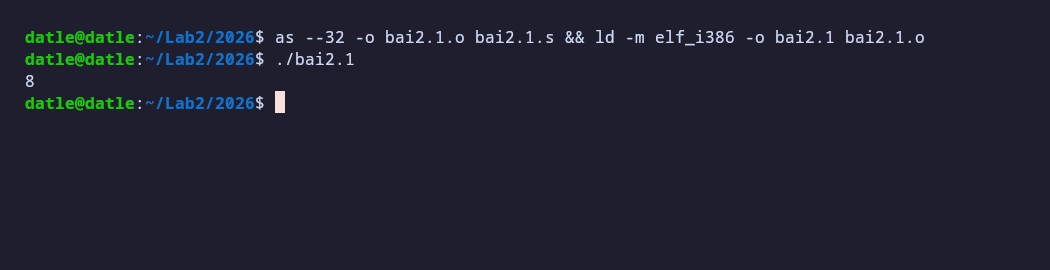
\includegraphics[width=0.88\textwidth]{images/terminal_bai2_1.png}
    \caption{Kết quả biên dịch, liên kết và thực thi Bài 2.1 (In độ dài chuỗi cho trước).}
    \vspace{0.4cm}
    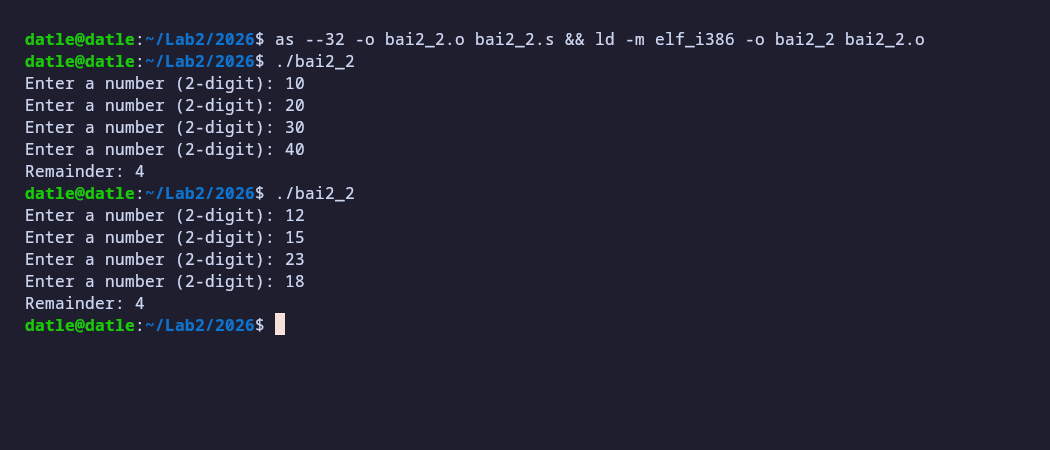
\includegraphics[width=0.88\textwidth]{images/terminal_bai2_2.png}
    \caption{Kết quả biên dịch, liên kết và thực thi Bài 2.2 (Số dư của tổng 4 số khi chia 8).}
\end{figure}

\newpage

\begin{figure}[h!]
    \centering
    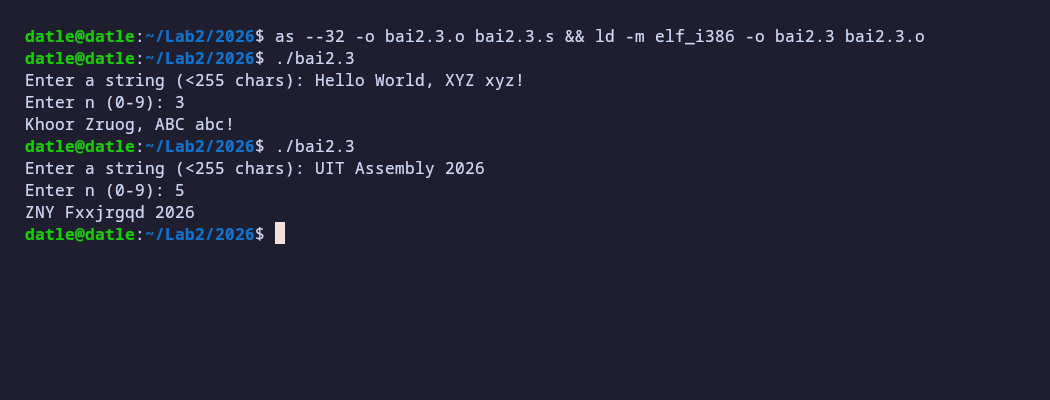
\includegraphics[width=0.88\textwidth]{images/terminal_bai2_3.png}
    \caption{Kết quả biên dịch, liên kết và thực thi Bài 2.3 (Mã hóa Caesar nâng cao 1 \& 2).}
    \vspace{0.4cm}
    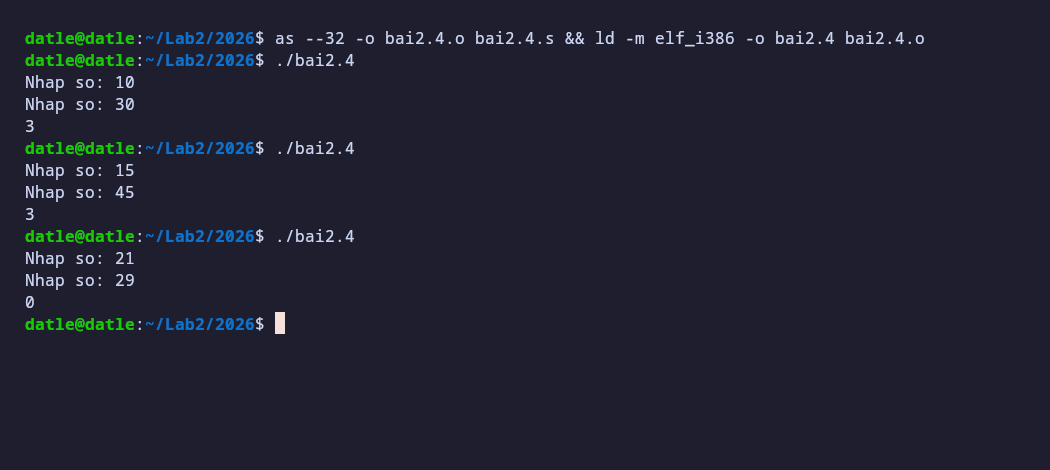
\includegraphics[width=0.88\textwidth]{images/terminal_bai2_4.png}
    \caption{Kết quả biên dịch, liên kết và thực thi Bài 2.4 (Đếm số lượng bội của 10 trong đoạn $[x, y]$).}
\end{figure}

\newpage

\begin{figure}[h!]
    \centering
    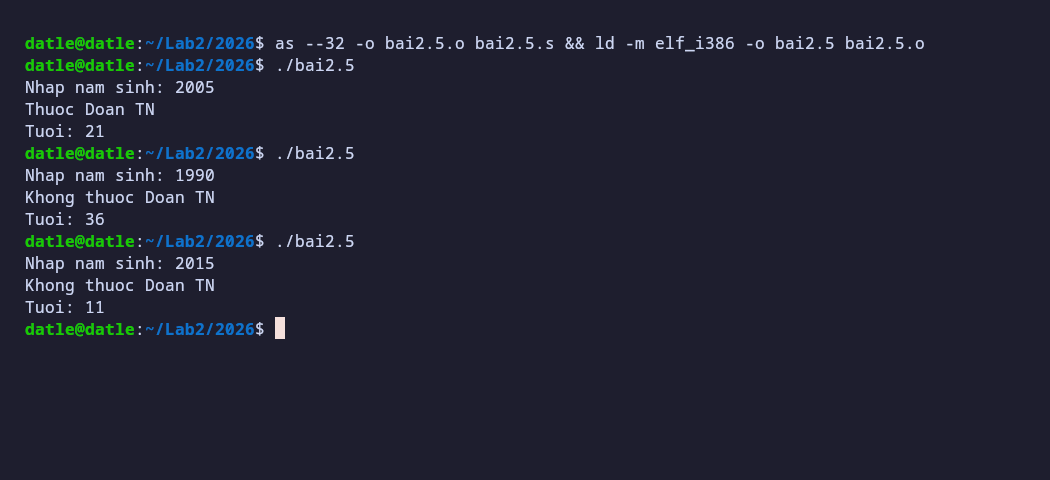
\includegraphics[width=0.88\textwidth]{images/terminal_bai2_5.png}
    \caption{Kết quả biên dịch, liên kết và thực thi Bài 2.5 (Kiểm tra tuổi đoàn và in kèm số tuổi).}
    \vspace{0.4cm}
    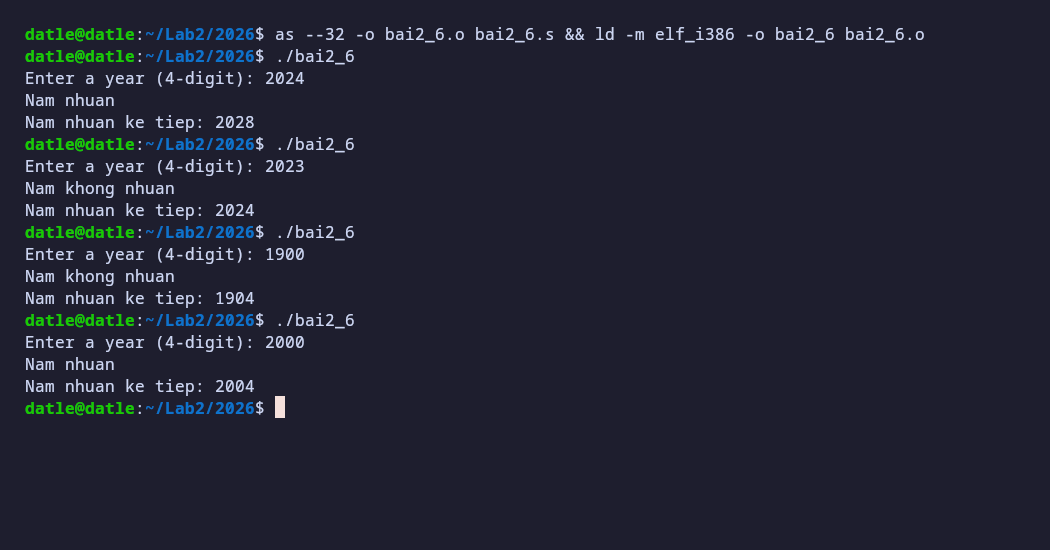
\includegraphics[width=0.88\textwidth]{images/terminal_bai2_6.png}
    \caption{Kết quả biên dịch, liên kết và thực thi Bài 2.6 (Kiểm tra năm nhuận và tìm năm nhuận kế tiếp).}
\end{figure}

\end{document}
